\begin{lstlisting}
from sie import *
\end{lstlisting}

\subsection{Beta Distribution Example}


\subsubsection{3 heads and 9 tails}


Plot a beta distribution with 3 heads and 9 tails...

\begin{lstlisting}
dist=beta(h=1,N=3)
distplot(dist,xlim=[0,1],show_quartiles=False)
\end{lstlisting}

\begin{center}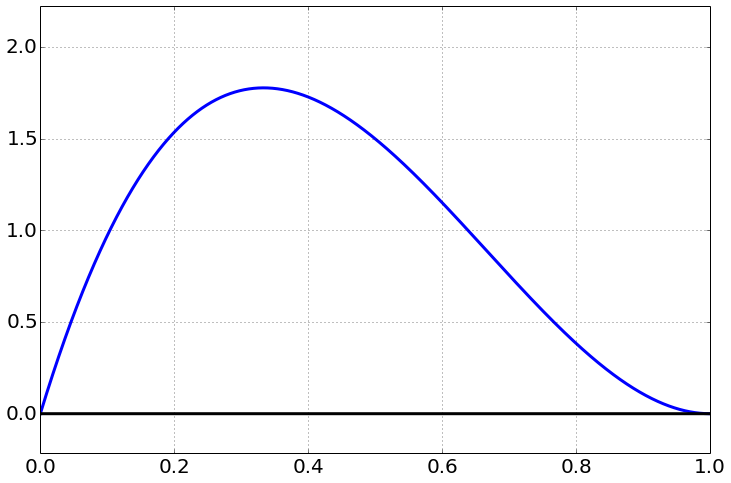
\includegraphics[width=4.5in]{Introduction_to_Parameter_Estimation/Introduction_to_Parameter_Estimation_fig0.png}\end{center}

The median of this distribution...

\begin{lstlisting}
dist.median()
\end{lstlisting}

\begin{verbatim}
0.27527583248615201
\end{verbatim}

the 95% credible interval, with the median in the middle,

\begin{lstlisting}
credible_interval(dist)
\end{lstlisting}

\begin{verbatim}
(0.067585986488542985, 0.38572756813238962, 0.80587955031675662)
\end{verbatim}

\subsubsection{1 heads and 3 tails}


This should be about the same fraction as the previous example, but broader

\begin{lstlisting}
dist=beta(h=1,N=4)
distplot(dist,xlim=[0,1])
\end{lstlisting}

\begin{verbatim}
<matplotlib.figure.Figure at 0x108768cd0>\end{verbatim}

\begin{center}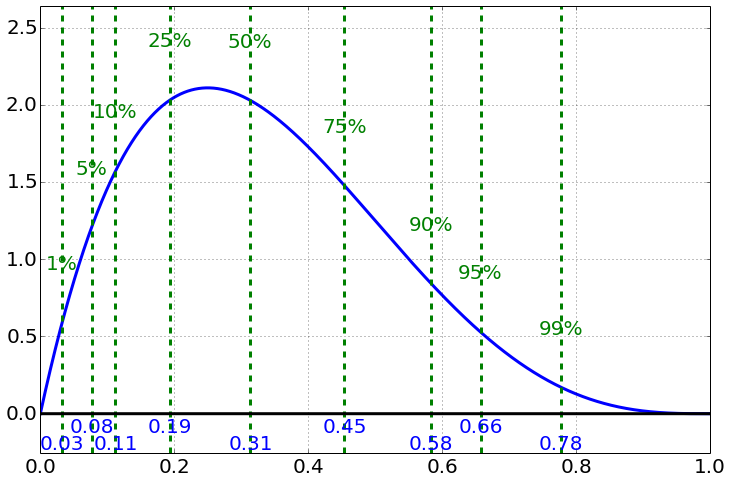
\includegraphics[width=4.5in]{Introduction_to_Parameter_Estimation/Introduction_to_Parameter_Estimation_fig1.png}\end{center}

\begin{lstlisting}
credible_interval(dist)
\end{lstlisting}

\begin{verbatim}
(0.052744950526316919, 0.31381017045569742, 0.71641793611808946)
\end{verbatim}

\begin{lstlisting}

\end{lstlisting}

